\documentclass[UTF8,fontset=fandol,11pt]{ctexart}
\usepackage[a4paper,margin=24mm,headheight=15pt]{geometry}
\usepackage{amsmath,amssymb,amsthm,mathtools,bm}
\usepackage{enumitem,booktabs,longtable,array,pdfpages,fancyhdr,xcolor}
\usepackage[colorlinks=true,linkcolor=blue!45!black,urlcolor=blue!45!black]{hyperref}
\allowdisplaybreaks[2]
\setlength{\parindent}{2em}
\setlength{\parskip}{3pt}
\setlength{\emergencystretch}{3em}
\setlist{nosep,topsep=3pt}
\pagestyle{fancy}\fancyhf{}\fancyhead[L]{\small 分析学讲义习题解答}\fancyhead[R]{\small 第38--57讲}\fancyfoot[C]{\thepage}
\newcommand{\R}{\mathbb R}\newcommand{\C}{\mathbb C}\newcommand{\N}{\mathbb N}\newcommand{\Z}{\mathbb Z}\newcommand{\Q}{\mathbb Q}\newcommand{\T}{\mathbb T}
\newcommand{\dd}{\,\mathrm d}\newcommand{\eps}{\varepsilon}\newcommand{\ind}{\mathbf1}
\newcommand{\norm}[1]{\left\lVert#1\right\rVert}\newcommand{\abs}[1]{\left|#1\right|}\newcommand{\ip}[2]{\left\langle#1,#2\right\rangle}
\DeclareMathOperator{\supp}{supp}\DeclareMathOperator{\rank}{rank}\DeclareMathOperator{\Span}{Span}\DeclareMathOperator{\diag}{diag}\DeclareMathOperator{\Res}{Res}\DeclareMathOperator{\Ext}{Ext}
\newcommand{\problem}[2]{\subsection*{#1}\addcontentsline{toc}{subsection}{#1}\noindent\textbf{题干。}#2\par\smallskip\noindent\textbf{解答。}}
\newcommand{\fix}[1]{\par\noindent\textcolor{red!55!black}{\textbf{原文核对与修正。}#1}\par}
\newcommand{\skipnote}[1]{\par\noindent\textbf{依约不解的计算题。}#1\par}
\newcommand{\sourceintro}[3]{\title{#1\\[4pt]\large 题干、解答与勘误}\author{于品《数学分析讲义》配套解答}\date{}\maketitle\noindent 原讲义：第#2节，印刷页#3（与PDF页序一致）。题干按数学内容重排；完整原题页附于文末，含未解的传统计算题，供逐字核对。原文中的作业提交说明及引文不作为本项目的工作指令。\par 本文中的“正函数”均按非负函数理解。复内积约定对第一个变量线性。}
\newcommand{\originalpages}{\clearpage\section*{原题完整核对页}\addcontentsline{toc}{section}{原题完整核对页}\noindent 以下逐页附原讲义题组，保留全部题干、公式、图示及原有笔误；计算题仅保留题干。\clearpage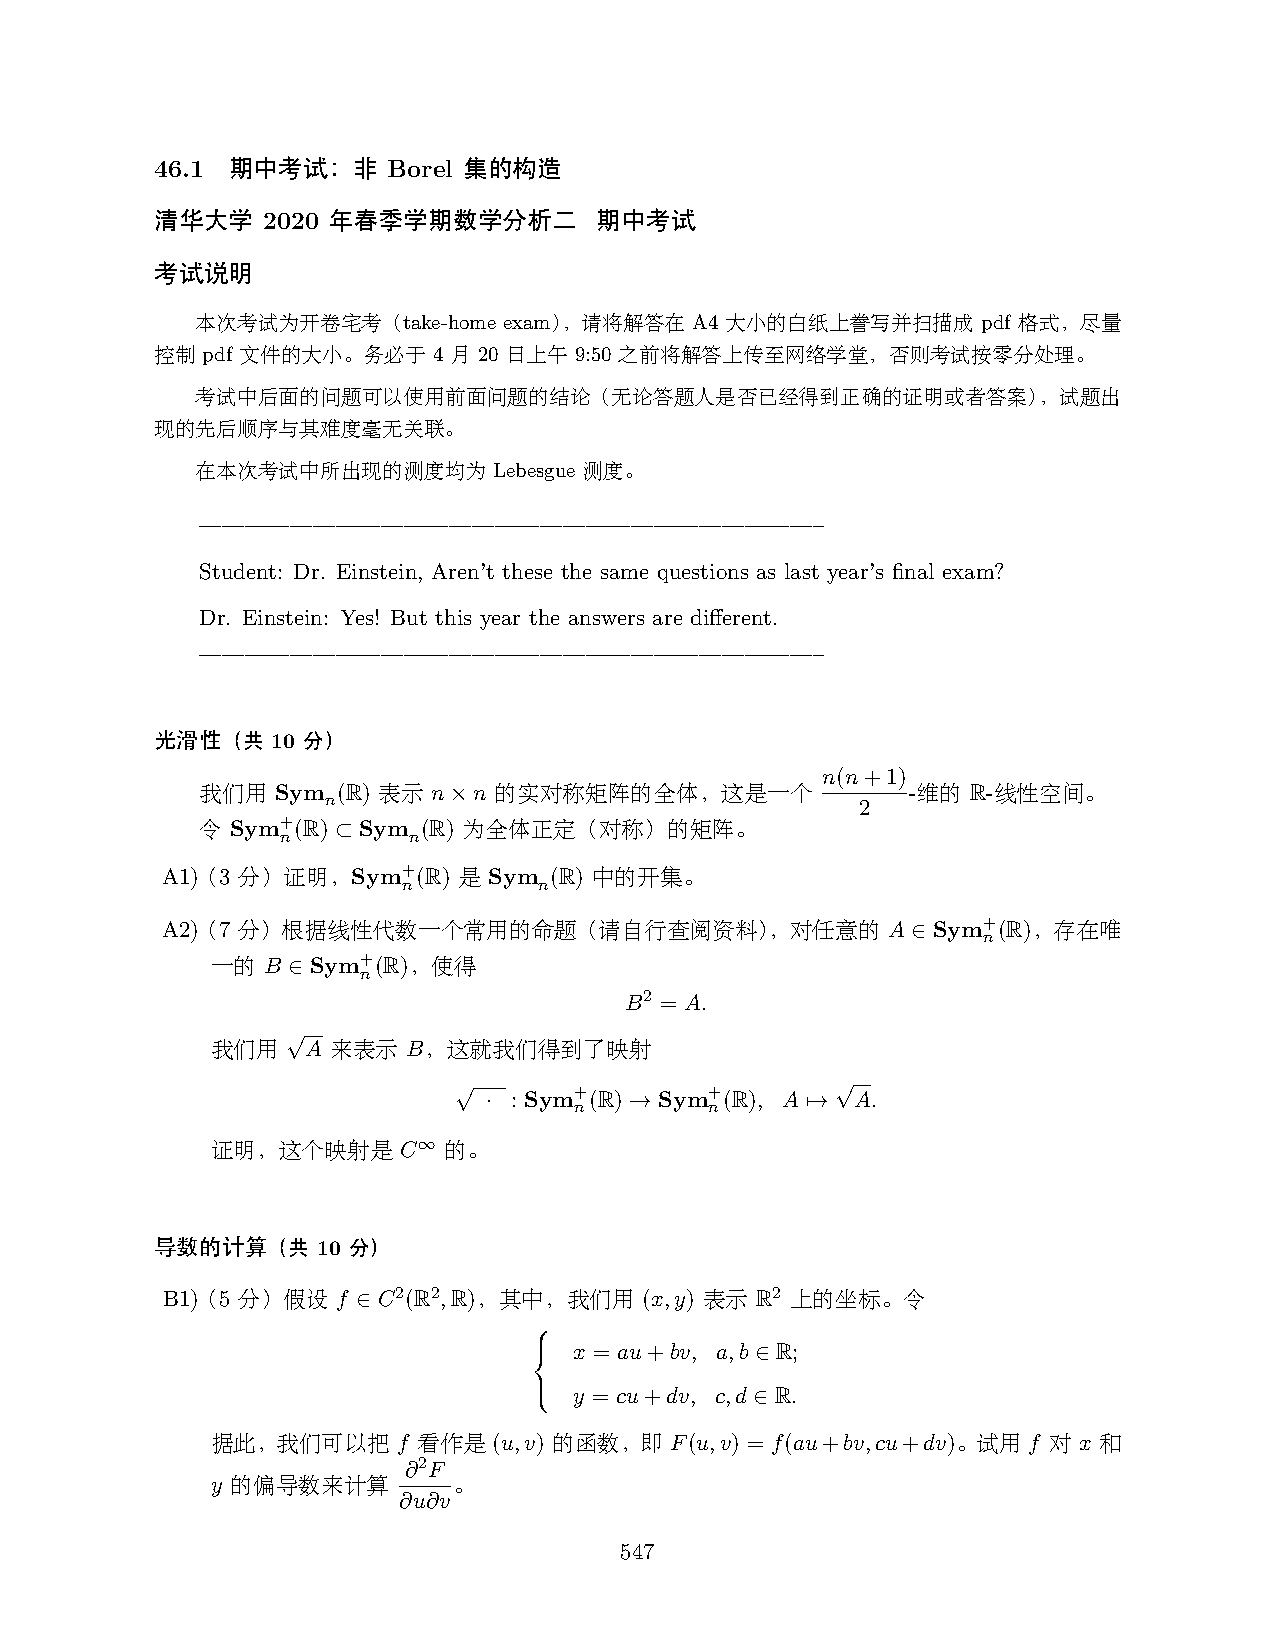
\includepdf[pages=-,pagecommand={\thispagestyle{empty}},scale=.94]{original.pdf}}

\begin{document}
\sourceintro{46.1 期中考试：光滑性、非Borel集与积分控制}{46.1}{547--552}
\section*{所用知识}
第31--37讲的微分、隐函数定理与凸性，第38--46讲的测度、控制收敛、Fubini及换元。正定矩阵只用实对称矩阵谱定理；Vitali集构造使用选择公理。I部分给出一致可积性的完整基础证明。
\section{正定矩阵的平方根}
\problem{A1}{证明$\operatorname{Sym}_n^+(\R)$在对称矩阵空间中是开集。}
对正定$A$，单位球上$x^TAx$的最小值$\lambda>0$。若$\norm H_{\rm op}<\lambda$且$H$对称，则$x^T(A+H)x\ge(\lambda-\norm H)|x|^2>0$。
\problem{A2}{已知正定对称矩阵$A$有唯一正定对称平方根$\sqrt A$，证明$A\mapsto\sqrt A$为$C^\infty$。}
考虑$\Psi(B)=B^2$在对称矩阵空间上的映射，$D\Psi_B(H)=BH+HB$。在正交基下$B=\diag(\lambda_i)$、$\lambda_i>0$，该导数将$H_{ij}$乘以$\lambda_i+\lambda_j$，故可逆。逆函数定理给出局部光滑逆；平方根的唯一性使各局部逆相容，得到全局光滑性。存在性由谱定理逐个取正平方根；唯一性也可由$B$与$B^2=A$交换并在$A$的各特征子空间上分析得到。
\section{微分方程与多项式根}
\skipnote{B1为线性坐标代换后混合偏导数的直接计算，不解；题干见附录第547页。}
\problem{B2}{找出所有$f\in C^2(\R^2,\R)$满足$f_{xx}-3f_{xy}+2f_{yy}=0$。}
令$u=x+y,v=2x+y$，写$f=F(u,v)$。因$\partial_x-\partial_y=\partial_v$、$\partial_x-2\partial_y=-\partial_u$，原算子为$-\partial_u\partial_v$，故$F_{uv}=0$。于是$F_u$与$v$无关，积分得$F(u,v)=A(u)+B(v)$，其中$A,B\in C^2(\R)$。反之直接代入成立。因此全部解为$f(x,y)=A(x+y)+B(2x+y)$。
令$P(a,b,x)=x^3+bx^2+ax+1$，$p_{a,b}(x)=P(a,b,x)$，$\Omega=\{(a,b):b^2<3a\}$。
\problem{C1}{证明$\Omega$开，且每个$p_{a,b}$在$\Omega$内有实根。}
$b^2-3a$连续，严格不等式定义开集。实首一三次多项式在$\pm\infty$分别趋于$\pm\infty$，介值定理给出实根，实际上此结论不需要参数在$\Omega$内。
\problem{C2}{对$(a,b)\in\Omega$的实根$x$，证明附近零点可由光滑函数$x'=\varphi(a',b')$唯一表示。}
$P_x=3x^2+2bx+a=3(x+b/3)^2+a-b^2/3>0$。隐函数定理直接给出所要求邻域与光滑函数。
\fix{原文等价条件的右边写成$x=\varphi(a',b')$，应为$x'=\varphi(a',b')$。}
\problem{C3}{若$p_{a,b}$有三个不同实根，证明参数充分小时仍有三个不同实根。}
三个根均为单根。在每个根上用隐函数定理，取三个互不交的小根邻域和公共参数邻域，得到三个不同实根分支。三次多项式不可能再有更多不同根。
\problem{C4}{证明$\Omega$内恰有一个实根。}
C2中的导数严格正，故多项式严格递增，再结合C1存在性。
\problem{C5}{令$U_1$为恰有一个实根的参数集合，$U_3$为有三个不同实根的集合。证明$U_1\cup U_3$在$\R^2$稠密。}
重根参数包含于判别式
\[D(a,b)=a^2b^2-4a^3-4b^3+18ab-27=0\]
的零点集。可由$P=P_x=0$消去$x$，或展开三次多项式判别式验证该式；$D(0,0)=-27$，所以非零。非零多项式的零点集无内点（逐变量运用一元多项式有限根性质即可），故其补集稠密。补集上的三次实多项式全是单根，实根数为一或三，因此包含于$U_1\cup U_3$。
\section{凸性与极值}
\problem{D1}{$\Omega$为内部非空的紧凸集，$f\in C(\Omega)\cap C^1(\Omega^\circ)$凸；若在内点$\omega$取到全局最大值，证明$f$常值。}
使用D3的证明即可，那里无需紧性或光滑性。
\problem{D2}{在闭单位圆盘上，令$f(\cos(1/n),\sin(1/n))=n$（$n\ge1$），其余为零。证明$f$凸且上确界为$+\infty$。}
这些特殊点互不相同，所以无界。对不同$x,y$和$0<t<1$，严格凸圆盘使$tx+(1-t)y$在开圆盘中，左边$f=0$，右边$tf(x)+(1-t)f(y)\ge0$；若$x=y$或$t=0,1$，不等式为等式。故凸性成立，即便边界上不连续。
\problem{D3}{只假设$\Omega$凸，$f$凸且在内点$\omega$达到全局上确界。证明对任意$x\in\Omega$有$f(x)=f(\omega)$。}
当$x\ne\omega$时取足够小$\eta>0$，$x'=\omega+\eta(\omega-x)\in\Omega$。有$\omega=\frac\eta{1+\eta}x+\frac1{1+\eta}x'$。两点函数值都不超过$f(\omega)$，凸不等式左端已为最大值，正权重迫使$f(x)=f(x')=f(\omega)$。
\problem{E1}{在非负八分空间定义$f(x,y,z)=xyz/(x+y+z)^2$，原点置零。证明连续，且在正八分空间$C^1$。}
原点外是分母不为零的光滑有理式。令$s=x+y+z$，由$xyz\le(s/3)^3$得$0\le f\le s/27\to0$，故原点连续。
\problem{E2}{对$a>0$，证明$f$在$K=\{x,y,z\ge0:x^2+y^2+z^2=a^2\}$达到最大值并求值。}
紧性与E1保证达到。边界值为零，而内部有正值，最大值在内部。对正变量有
\[(x+y+z)^2\ge3(xy+yz+zx),\quad (xy+yz+zx)^2\ge3xyz(x+y+z).\]
另一种便于确定等号的办法是拉格朗日：$\log f$的偏导为$1/x-2/s$，故在极值处$1-2x/s=2\lambda x^2$，另两变量同理。三式相加得$1=2\lambda a^2$，所以$\lambda>0$。若$x\ne y$，相减并除以$x-y$得$-2/s=2\lambda(x+y)>0$，矛盾。因此$x=y=z=a/\sqrt3$，最大值为$a/(9\sqrt3)$。本小问保留其不等式和极值论证。
\section{Hopf纤维化}
\problem{F1}{证明$S^3\subset\R^4$与$S^2\subset\R^3$是光滑子流形。}
各自是$|x|^2=1$的正则水平集，因为梯度$2x$不为零。
\problem{F2}{令$H(x,y,z,w)=(x^2+y^2-z^2-w^2,2(xw+yz),2(yw-xz))$。证明$H(S^3)\subset S^2$且每个纤维为$S^3$的子流形。}
\fix{原文把该三分量映射的值域写成$\R^2$，应为$\R^3$。}
展开得$|H(p)|^2=|p|^4$。Jacobi矩阵的三行两两正交、每行平方长为$4|p|^2$，所以$DH_pDH_p^T=4I_3$在$S^3$上成立。又$DH_p p=2H(p)$。给定$v\perp H(p)$，取$u=DH_p^Tv/4$，有$u\perp p$且$DH_pu=v$。故$H|_{S^3}$为到$S^2$的淹没，正则水平集定理使每个非空纤维为一维子流形；非空性见F3的显式构造。
\problem{F3}{证明每个$H^{-1}(a,b,c)$与单位圆周微分同胚。}
令$u=x+iy,v=z+iw$，则$|u|^2=(1+a)/2$、$|v|^2=(1-a)/2$、$uv=(-c+ib)/2$。若$a>-1$，写$u=r e^{it}$，$r=\sqrt{(1+a)/2}>0$，则$v=(-c+ib)e^{-it}/(2r)$。这给出圆周到纤维的光滑双射，其逆为$u/r$，也光滑。若$a=-1$，则$b=c=0,u=0,|v|=1$，结论同样明显。
\section{非Borel集}
\problem{G1}{在$[0,1]$上以$x\sim y\iff x-y\in\Q$分等价类，每类选一点组成$A$。对$q\in[-1,1]\cap\Q$令$A_q=A+q$。验证等价关系，并证明不同平移不相同，且$[0,1]\subset\bigcup_qA_q\subset[-1,2]$。}
有理数加法群给出自反、对称、传递性。实际上不同平移两两不交：若$a+q=a'+q'$，则$a\sim a'$，代表唯一性给出$a=a'$进而$q=q'$。对$x\in[0,1]$，其代表$a$满足$x-a\in[-1,1]\cap\Q$，故被覆盖；外侧包含显然。
\problem{G2}{证明$A$不是Borel集。}
若可测，所有$A_q$等测度且两两不交。若$m(A)=0$，其可数并不能覆盖测度为$1$的区间；若$m(A)>0$，可数并测度为无穷，却包含于$[-1,2]$，均矛盾。事实上证明了它不Lebesgue可测。
\problem{G3}{若$\mu$是$\mathcal P(\R)$上平移不变测度，证明要么恒零，要么每个非空开区间都有无穷测度。}
若某个非空开区间$I$的测度有限，则将$[0,1]$经平移缩放式的有限覆盖（只需平移长度小于$|I|$的子区间）可知每个有界区间测度有限。对G1的代表集及平移使用相同不交论证，有限性迫使$\mu(A)=0$，从而$\mu([0,1])=0$。整数平移覆盖全直线，给出$\mu(\R)=0$。否则每个非空开区间必为无穷。
\section{含参数的Gauss型积分}
令$a>0$，$H_a(x)=\int_0^\infty e^{-at^2-x/t^2}\dd t$，$x\ge0$。
\problem{H1}{证明积分良定义并计算$H_a(0)$。}
被积函数由$e^{-at^2}$控制，故绝对可积。由第44讲Gauss积分，$H_a(0)=\sqrt\pi/(2\sqrt a)$。
\problem{H2（连续性）}{证明$H_a:[0,\infty)\to\R$连续。}
对每个$t>0$参数连续，仍用$e^{-at^2}$控制，应用控制收敛，包括$x=0$。
\problem{H2（可微性，原题重号）}{证明$H_a$在$(0,\infty)$可微。}
在$x\in[b,c]\subset(0,\infty)$上，导数绝对值由$t^{-2}e^{-at^2-b/t^2}$控制，它在零点指数衰减、无穷远可积，故可在积分号下求导。
\problem{H3}{计算$H_a'(x)$。}
$H_a'(x)=-\int_0^\infty t^{-2}e^{-at^2-x/t^2}\dd t$。换元$t=\sqrt{x/a}/u$得到$H_a'(x)=-\sqrt{a/x}\,H_a(x)$。
\problem{H4}{证明$H_a(x)=\frac12\sqrt{\pi/a}\,e^{-2\sqrt{ax}}$。}
对$x>0$解H3的一阶方程，得到$H_a(x)=Ce^{-2\sqrt{ax}}$，H2与H1确定$C=\sqrt\pi/(2\sqrt a)$，且公式延续至零点。本组保留以展示积分求导与反常端点控制。
\section{积分控制与一致可积性}
设$f\in L^1(\Omega)$，$\Omega\subset\R^n$可测。
\problem{I1}{证明$\int_\Omega|f|\ind_{\{|x|\ge R\}}\dd x\to0$。}
示性函数逐点趋零，以$|f|$控制。
\problem{I2}{证明$\int_\Omega|f|\ind_{\{|f|\ge R\}}\dd x\to0$。}
可积函数有限几乎处处，仍用控制收敛。
\problem{I3}{证明对每个$\eps>0$存在$\delta>0$，当$m(A)<\delta$时$\int_A|f|<\eps$。}
取$R$使I2的尾项$<\eps/2$，再令$\delta=\eps/(2R)$，有$\int_A|f|\le Rm(A)+\int_{|f|\ge R}|f|<\eps$。
以下$m(\Omega)<\infty$，每个$f_k\in L^1(\Omega)$。
\problem{I4}{假设$\lim_{R\to\infty}\sup_k\int_{|f_k|\ge R}|f_k|=0$。证明I3可对全体$f_k$使用同一个$\delta$。}
按I3相同分解，选使所有尾项小于$\eps/2$的统一$R$即可。
\problem{I5}{反过来，假设积分关于小测度集合一致绝对连续，证明$\lim_{R\to\infty}\sup_k\int_{|f_k|\ge R}|f_k|=0$。}
先证明$M=\sup_k\norm{f_k}_1<\infty$：对$\eps=1$取$\delta$，将$\Omega$分成有限个测度$<\delta$的可测块。可先取大盒使盒外质量$<\delta$，盒内用体积$<\delta$的有限网格切分。每块上积分至多$1$，故有统一界$M$。给定$\eps$再取其对应$\delta_\eps$，由Chebyshev不等式$m(|f_k|\ge R)\le M/R<\delta_\eps$，便得到所有尾积分小于$\eps$。
\problem{I6}{假设$f_k\to f$逐点，且满足I4或I5的假设。证明$\int|f_k-f|\to0$。}
\fix{原文引用“H4或H5”，应为“I4或I5”。}
统一$L^1$界和Fatou使$f\in L^1$；对每个可测$A$，Fatou又给出$\int_A|f|\le\liminf_k\int_A|f_k|$，故同一个小集合控制也适用于$f$。对$\eta>0$，$E_k=\{|f_k-f|>\eta\}$的测度趋零：它包含于$\bigcup_{j\ge k}E_j$，这些尾部并集在忽略一个零测集后递减到空，利用有限测度的从上连续性。于是
\[\int|f_k-f|\le\eta m(\Omega)+\int_{E_k}(|f_k|+|f|).\]
先取$\eta$小，再由一致绝对连续性使第二项小，得到结论。
\originalpages
\end{document}
